% vim: set ft=tex:

\section{Introduction}
In software development, there are several critical steps that must be followed in order to create a successful software application. Among these steps are the analysis and design phases. The analysis phase involves gathering requirements and understanding the needs of the users and stakeholders. This phase is crucial because it lays the foundation for the design phase, which involves creating a plan for how the software will be built and what it will do.



\section{Scope Statement}
A blood donation app is a mobile application designed to connect blood donors with blood banks and hospitals to facilitate blood donations. The app allows users to register as donors, search for nearby blood banks and hospitals in need of donations, schedule appointments, and track their donation history. The aim of the project is to increase access to blood donations and make the donation process more convenient for both donors and recipients.

\begin{itemize}
\item \textbf{Project Objective:} The objective of this project is to design and develop a mobile application that allows individuals to easily schedule appointments to donate blood in nearby blood banks and hospitals, and track their donation history.
\item \textbf{Project Deliverables: }The project will deliver a fully functional mobile application for Android devices. The application will include features such as user registration, appointment scheduling, donation tracking, and notifications for blood banks and hospitals in need of donations.
\item \textbf{Project Boundaries:} The project will include the development of the mobile application and any necessary server-side components. The project will not include the physical collection or transportation of blood.
\item \textbf{Project Constraints:} The project must be completed within a budget of 200000 DA and a timeframe of 2 months.
\item \textbf{Project Assumptions: } The project assumes that there is a need for a blood donation app, that potential users have access to smartphones and the internet, and that there are a sufficient number of blood banks and hospitals interested in using the app.
\item \textbf{Project Sub Functions:} 
\begin{itemize}
\item  User registration
\item  Profile management
\item Appointment scheduling
\item  Donation tracking (history of donations)
\item  Notifications for blood banks and hospitals
\end{itemize}
\item \textbf{Actors(Stakeholders):} 
\begin{itemize}
\item \textbf{Donor:}  the application allows the donor to:
\begin{itemize}
\item  Authantificate 
\item  Make donation
\item See content about blood donation process
\item  Check the tests result
\item  Check the history of donations
\item  Check his profile
\item  Edit / delete profile
\item  Receive notifications
\end{itemize}
\item \textbf{Admin:}  The admin is able to use the application to:
\begin{itemize}
\item  Authenticate 
\item  See content about blood donation process
\item Send test result
\item  Send notifications
\end{itemize}
\item \textbf{Guest:}  guests are able to:
\begin{itemize}
\item  Register 
\item  See content about blood donation process
\end{itemize}
\end{itemize}
\end{itemize}


\section{Unified Modeling Language(UML)}


\subsection{Definition}
Unified Modeling Language (UML) is a standardized visual language used in software engineering to document, design, and analyze software systems. It provides a common language for understanding and describing the different aspects of a software system through diagrams and models.

\begin{figure}[H]
    \centering
    
\includegraphics[width=0.5\textwidth]{images/UML_logo.svg.png}
    \caption{UML logo}
    \label{fig:figure4}
\end{figure}
\subsection{UML Advantages}

\begin{itemize}
\item  Helps in communication
\item   Help developers save time by automating some of the design processes
\item Allows different software developers to work on the same project
\item  Provides a better understanding of a system
\item  Unifies design by providing a standard way to design software and systems
\end{itemize}


\section{Use Case Diagram}
\subsection{Definition}
A use case diagram is a type of UML diagram used to model the interactions between users (actors) and a system, showing how the system responds to user actions or requests. It consists of actors, use cases, and relationships between them, and is useful for capturing and communicating system requirements.

\subsection{Use case diagram of the Application}

in our application we have identified three key actors in which each has a role: Admin, Donor, Guest.

\begin{figure}[H]
    \centering
    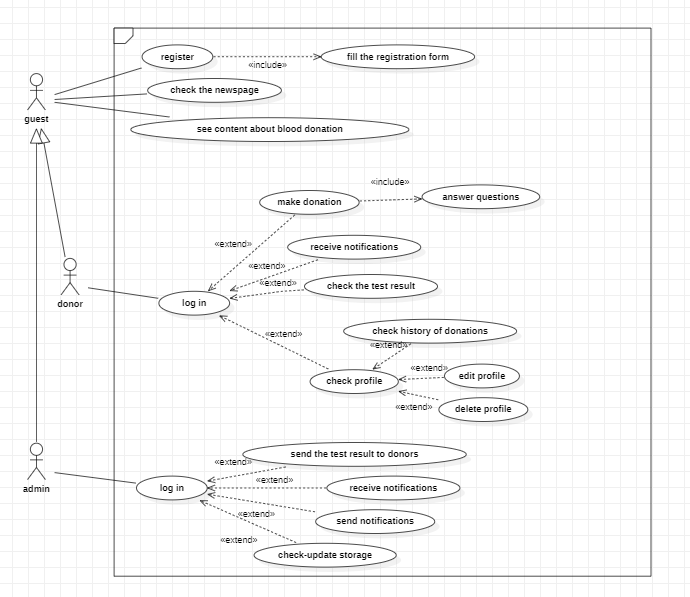
\includegraphics[width=1\textwidth]{images/use.png}
    \caption{Use Case Diagram}
    \label{fig:figure4}
\end{figure}



\section{Class Diagram}
\subsection{Definition}
A class diagram is a UML diagram used to model the structure of a system by showing the classes, attributes, methods, and relationships between them. It represents the static view of the system and provides a blueprint for the implementation of the system. Class diagrams are useful for visualizing and organizing complex systems in the design phase of software development.
\subsection{Class diagram of the application}

\begin{figure}[H]
    \centering
    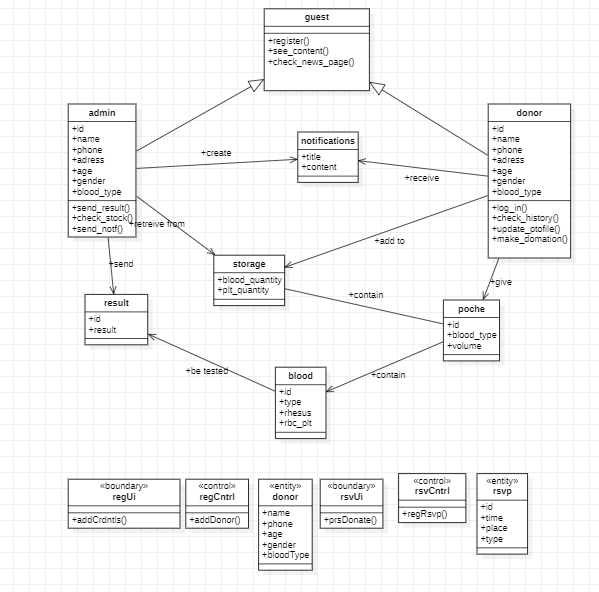
\includegraphics[width=1\textwidth]{images/niw.png}
    \caption{ Class Diagram}
    \label{fig:figure4}
\end{figure}

\section{Sequence Diagram}
\subsection{Definition}
A sequence diagram is a type of UML diagram used in software engineering to model the interactions between objects or components in a system. It represents a dynamic view of the system by showing the sequence of messages exchanged between objects and the order in which they occur. Sequence diagrams are useful for analyzing and designing systems that have complex interactions between different components or objects.
\subsection{Use Case Description}

\begin{figure}[H]
    \centering
    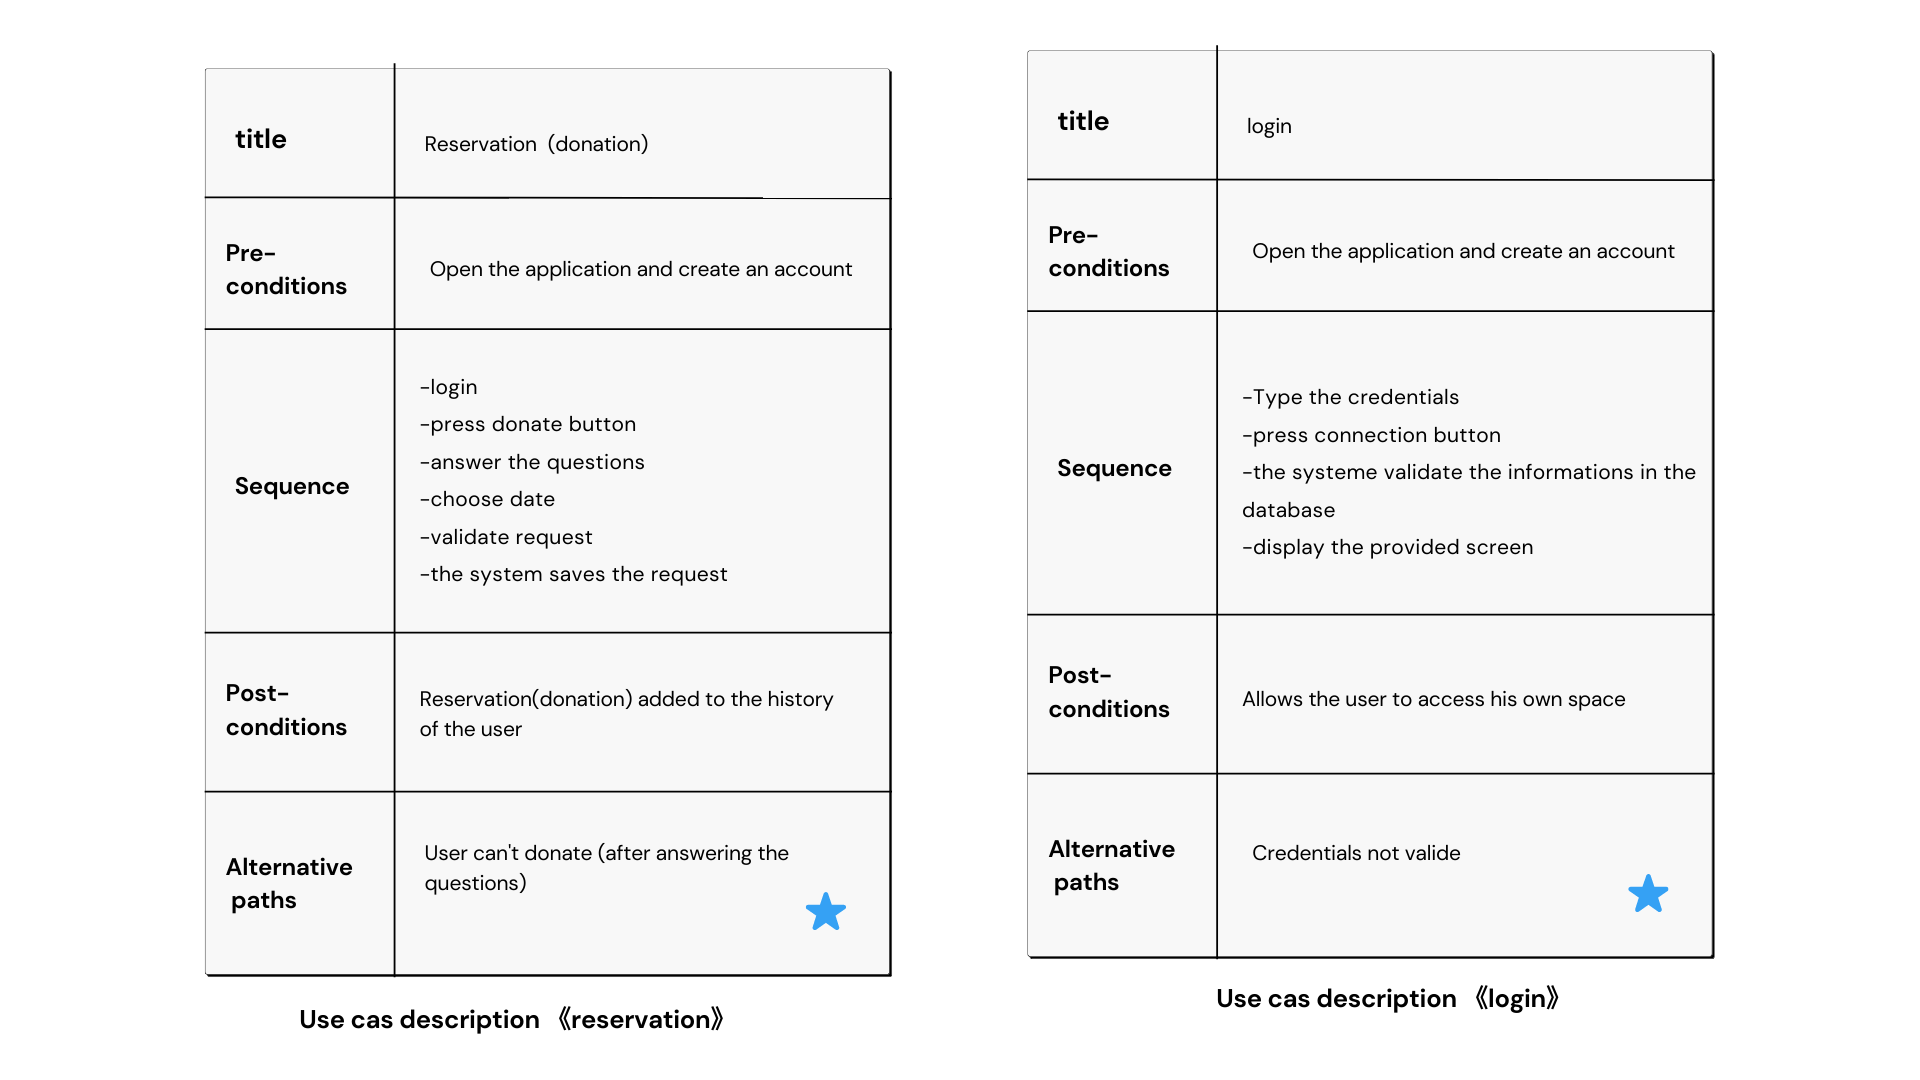
\includegraphics[width=1\textwidth]{images/Let's brainstorm for thoughts, ideas, and inspiration using an idea board..png}
    \caption{Use Case description}
    \label{fig:figure4}
\end{figure}
\subsection{Sequence Diagram of the Application}

\begin{figure}[H]
    \centering
    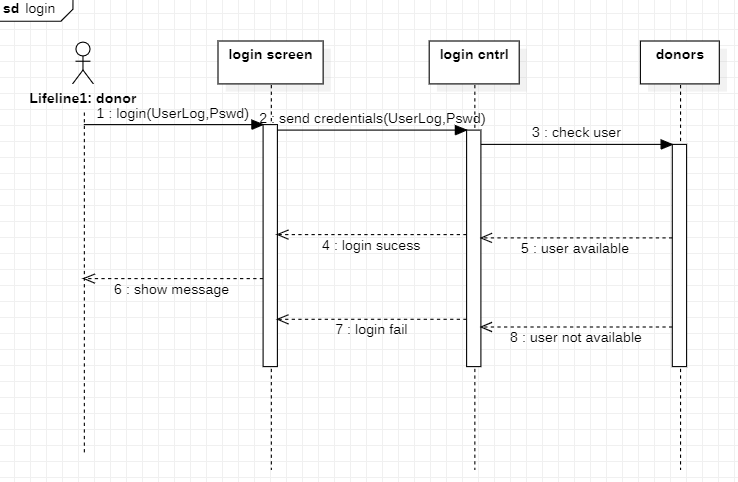
\includegraphics[width=1\textwidth]{images/login.png}
    \caption{ Login Sequence Diagram}
    \label{fig:figure4}
\end{figure}

\begin{figure}[H]
    \centering
    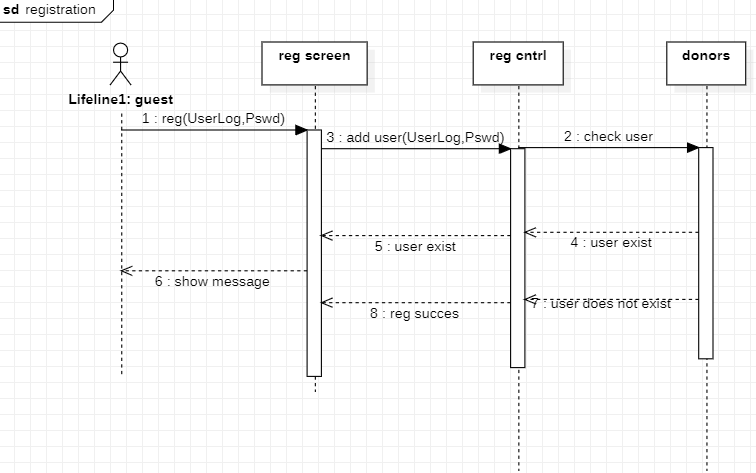
\includegraphics[width=1\textwidth]{images/regs.png}
    \caption{Registration Sequence Diagram}
    \label{fig:figure4}
\end{figure}

\begin{figure}[H]
    \centering
    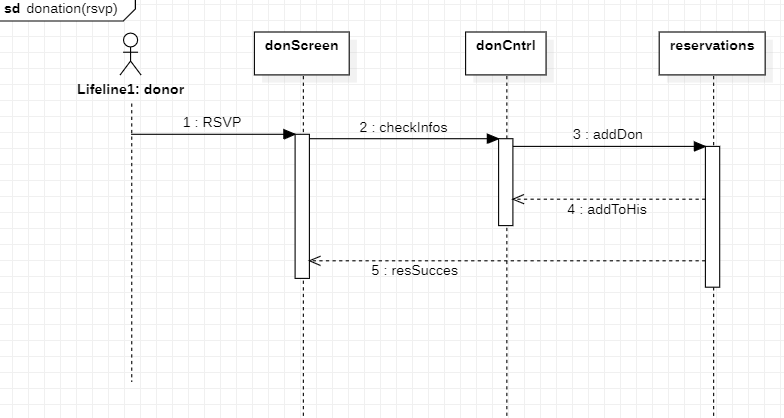
\includegraphics[width=1\textwidth]{images/don.png}
    \caption{Make Donation Sequence Diagram}
    \label{fig:figure4}
\end{figure}


%\section{Conclusion}

%that included various UML diagrams, including use case diagrams, %diagram classes, and sequence diagrams.

%The suggested conceptual solution will be presented in the following %chapter.

